\documentclass[border=4pt]{standalone}
% shared style for all PyTBA topology diagrams (\input by each standalone file)
\usepackage{mathpazo}
\usepackage{amsmath}
\usepackage{tikz}
\usetikzlibrary{positioning,arrows.meta,calc,decorations.pathreplacing,fit,backgrounds}
\tikzset{
  host/.style={draw=blue!55!black, fill=blue!7, rounded corners=2pt, align=center,
               minimum height=9mm, minimum width=22mm, font=\small},
  blk/.style={draw=black!60, fill=black!4, rounded corners=2pt, align=center,
              minimum height=8mm, font=\small},
  chan/.style={draw=orange!70!black, fill=orange!8, rounded corners=2pt, align=center,
               minimum height=9mm, font=\small},
  lossbox/.style={draw=red!70!black, fill=red!6, rounded corners=2pt, align=center, font=\footnotesize},
  data/.style={-{Stealth[length=2.2mm]}, thick},
  ack/.style={-{Stealth[length=2mm]}, dashed, black!60},
  lbl/.style={font=\footnotesize, align=center},
  brace/.style={decorate, decoration={brace, amplitude=4pt}, thick, black!70},
}

\begin{document}
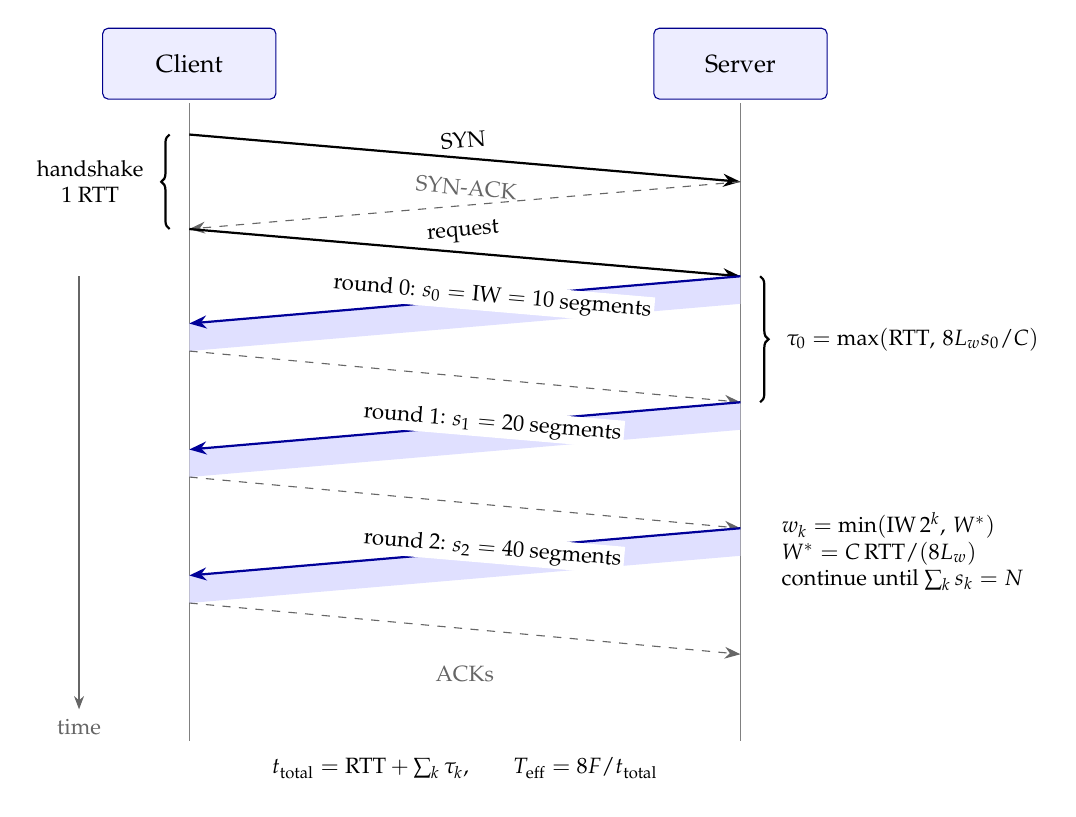
\begin{tikzpicture}[yscale=-1]
\node[host] (c) at (0,0) {Client};
\node[host] (s) at (7,0) {Server};
\draw[black!50] (0,0.5) -- (0,8.6); \draw[black!50] (7,0.5) -- (7,8.6);
% handshake and request
\draw[data] (0,0.9) -- node[lbl, above, sloped] {SYN} (7,1.5);
\draw[ack]  (7,1.5) -- node[lbl, above, sloped] {SYN-ACK} (0,2.1);
\draw[data] (0,2.1) -- node[lbl, above, sloped] {request} (7,2.7);
\draw[decorate, decoration={brace, amplitude=3pt, mirror}, thick] (-0.25,0.9) -- node[lbl, left=2mm] {handshake\\1 RTT} (-0.25,2.1);
% slow-start rounds
\foreach \k/\y/\n in {0/2.7/{\mathrm{IW}=10}, 1/4.3/{20}, 2/5.9/{40}} {
  \fill[blue!12] (7,\y) -- (7,\y+0.35) -- (0,\y+0.95) -- (0,\y+0.6) -- cycle;
  \draw[data, blue!60!black] (7,\y) -- node[lbl, sloped, black, fill=white, inner sep=1pt, pos=0.45] {round $\k$: $s_\k=\n$ segments} (0,\y+0.6);
  \draw[ack] (0,\y+0.95) -- (7,\y+1.6);
}
\node[lbl, black!60] at (3.5,7.75) {ACKs};
\draw[decorate, decoration={brace, amplitude=3pt}, thick] (7.25,2.7) -- node[lbl, right=2mm] {$\tau_0=\max(\mathrm{RTT},\,8L_w s_0/C)$} (7.25,4.3);
\node[lbl, align=left, anchor=west] at (7.4,6.2) {$w_k=\min(\mathrm{IW}\,2^k,\,W^*)$\\$W^*=C\,\mathrm{RTT}/(8L_w)$\\continue until $\sum_k s_k=N$};
\draw[-{Stealth}, black!60] (-1.4,2.7) -- (-1.4,8.2) node[lbl, below] {time};
\node[lbl] at (3.5,8.95) {$t_{\mathrm{total}}=\mathrm{RTT}+\sum_k\tau_k$,\qquad $T_{\mathrm{eff}}=8F/t_{\mathrm{total}}$};
\end{tikzpicture}
\end{document}
